\scanpage{4}
\deleted{\unsure{Recall|Recall}}

\uline{Graphs}

\[
\begin{aligned}
\text{\uline{Definition}}\\[-2pt]\text{\uline{\unsure{Graph|Graphs}}}
\end{aligned}
\quad
\left\{\begin{aligned}
&\text{Set } S\ \text{of ``vertex''}\\
&\text{set } A\ \text{``of edges''}\\
&R\subset S\times A\qquad\text{incidence relation}
\end{aligned}\right\}
\ \text{Data}
\]

\uline{\unsure{Axiom|Axioms}} \quad 1) $\forall a\in A,\ \unsure{\exists|\exists s}\ \operatorname{card}R\{a\}=2$ (every edge has exactly 2 vertices)

\noindent\begin{minipage}[t]{.32\linewidth}
\figure{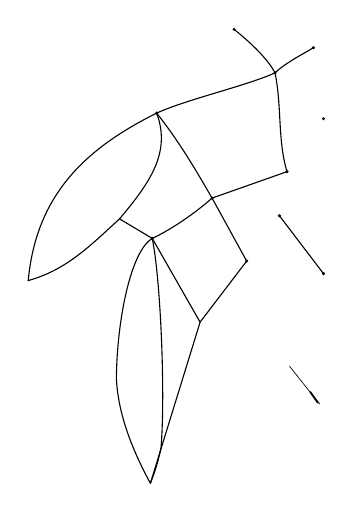
\begin{tikzpicture}[x=.008cm,y=-.008cm,line cap=round,line join=round]
\draw (492,496) .. controls (511,511) and (544,540) .. (557,565)
  .. controls (575,548) and (604,534) .. (618,525);
\draw (557,565) .. controls (514,585) and (417,607) .. (369,629)
  .. controls (263,682) and (178,753) .. (165,895);
\draw (165,895) .. controls (226,878) and (263,840) .. (310,797)
  .. controls (359,739) and (392,691) .. (369,629);
\draw (369,629) .. controls (404,673) and (431,719) .. (457,764)
  -- (576,722) .. controls (561,672) and (568,619) .. (557,565);
\draw (310,797) -- (362,828) .. controls (394,813) and (431,787) .. (457,764)
  -- (512,864) -- (438,961) -- (362,828);
\draw (362,828) .. controls (328,848) and (306,957) .. (305,1050)
  .. controls (308,1116) and (338,1178) .. (359,1217);
\draw (362,828) .. controls (375,891) and (383,1071) .. (376,1160)
  .. controls (371,1185) and (365,1202) .. (359,1217);
\draw (438,961) -- (359,1217);
\draw (564,792) -- (634,884);
\draw[line width=.25pt] (580,1031) .. controls (593,1047) and (609,1068) .. (628,1091);
\draw[line width=.65pt] (613,1072) -- (625,1089);
\foreach \x/\y in {492/496,618/525,557/565,369/629,576/722,457/764,362/828,512/864,564/792,634/884,634/638}
  \fill (\x,\y) circle[radius=2.7];
\end{tikzpicture}}
\end{minipage}\hfill
\begin{minipage}[t]{.63\linewidth}
A graph is called \deleted{\unsure{quelq.|something}} \uline{strict} if an edge is known when one knows its vertices.

\deleted{\unsure{One|A|A}} The datum of a \uline{strict graph} is therefore equivalent \unsure{to the|to 2} datum of a set $S$, and of a subset $A$ of $\mathfrak{P}_{2}(S)$ (set of subsets of cardinality 2 of $S$).
\end{minipage}

Arc of a graph (or oriented edge) -- set $\vec A$

\deleted{\uline{\unsure{Remark}}} Topological realization of a graph
\[
\deleted{X(S,A,R)=\bigl(S\amalg(\vec A\times I)\bigr)/.}
\]

a) Segment associated to a set $a$ of cardinality 2
\[
\begin{aligned}
\bigl[\,\deleted{\unsure{\operatorname{réal}|\operatorname{rel}}}\inserted{\operatorname{seg}}(a)&\subset I^{a}\qquad (I=[0,1])\\
\operatorname{seg}(a)&=\bigl\{\{t_{\unsure{x|n}}\}_{x\in a}\mid\textstyle\sum t_x=1\bigr\}\ ;\ \text{one has }\ a\hookrightarrow\operatorname{seg}(a)
\end{aligned}
\]

b)
\[
\operatorname{réal}(S,A,R)\unsure{=|\equiv}\left(S\amalg\coprod_{a\in A}\operatorname{seg} R\{a\}\right)\big/\begin{aligned}&\text{equivalence}\\&\text{relation}\end{aligned}
\]

\deleted{\unsure{Realization}} \quad [ \unsure{If|One|If one} has $X=\coprod_{a\in A}\operatorname{seg}R\{a\}$, one has
\diagram{\begin{tikzcd}[ampersand replacement=\&,row sep=0.2em,column sep=1.7em]
\partial X \arrow[r] \& S\\[-2pt]
\cap \& {}\\[-2pt]
X \& {}
\end{tikzcd}}
and one ``attaches'' $X$ \unsure{to|:} $S$ \unsure{by|by|$\vdash$} $\partial X\to S$ \quad ]

``Rectilinear \inserted{geometric} realization'' of a graph (finite..) in a vector space (of finite dimension\ldots) over $\mathbb{R}$ : homeomorphism into
% archive sheet number: 3
